\section{Master-Theorem}

\begin{frame}{Teile und herrsche -- divide and conquer}
	\daniel{Manchmal sind wir zu faul, große Probleme alleine anzupacken...}
	\begin{itemize}
		\item Probleminstanz in kleinere Teile \textbf{zerlegen}
		\item \thassedaniel{Teile rekursiv nach gleichen Verfahren bearbeiten}{Für jeden Teil \textbf{klonen} wir uns einmal und lassen den Klon die Arbeit machen \\
		{\small (Der Klon ist natürlich genauso faul wie wir und klont sich ebenfalls)}}
		\item \thassedaniel{Aus Teilergebnissen Resultat rekonstruieren}{Ergebnisse von den Klonen \textbf{einsammeln} und \textbf{zusammenfügen}}
	\end{itemize}
\end{frame}

\begin{frame}{Das Master-Theorem (einfache Form)}
	Situation aus dem Leben: 
	\begin{itemize}[<+->]
		\item Wir haben einen rekursiven Algorithmus $A$ für ein Problem der Größe $n$
		\item Bei jedem Schritt wird das Problem durch $b$ \textbf{geteilt} und es ergeben sich $d$ neue Probleminstanzen der Größe $n/b$
		\item \thassedaniel{Aufteilen}{Klonen} und Ergebnisse zusammentragen geht in $c \· n$ Operationen (für konstantes $c$)
		%\item Wir können die Laufzeit der jeweiligen \enquote{Auseinandernehmungs-} und \enquote{Zusammenführungsschritte} \textbf{linear} abschätzen.
	\end{itemize}
\end{frame}

\begin{frame}{Das Master-Theorem (einfache Form)}  % TODO Überarbeitung von hier wieder in Algotutfolien übertragen!
	Seien $a, \textcolor{blue}{b}, c, \textcolor{darkgreen}{d}$ positive Konstanten und für $n \in \N$ sei 
	\[
	T(n) = 
	\begin{cases}
	a,  & \text{für } n = 1 \\
	\textcolor{darkgreen}{d} \cdot T\large(\frac{n}{\textcolor{blue}{b}}\large) + c\·n, & \text{für } n > 1
	\end{cases}
	\]
	gegeben. \\ \smallskip
	
	Dann gilt:
	\[
	T(n) \in 
	\begin{cases}
	\Th{n},                                                        & \textcolor{darkgreen}{d} < \textcolor{blue}{b} \\
	\Th{n \log n},                                                 & \textcolor{darkgreen}{d} = \textcolor{blue}{b} \\
	\Th{n^{\log _{\textcolor{blue}{b}} \textcolor{darkgreen}{d}}}, & \textcolor{darkgreen}{d} > \textcolor{blue}{b}
	\end{cases}.
	\]
	%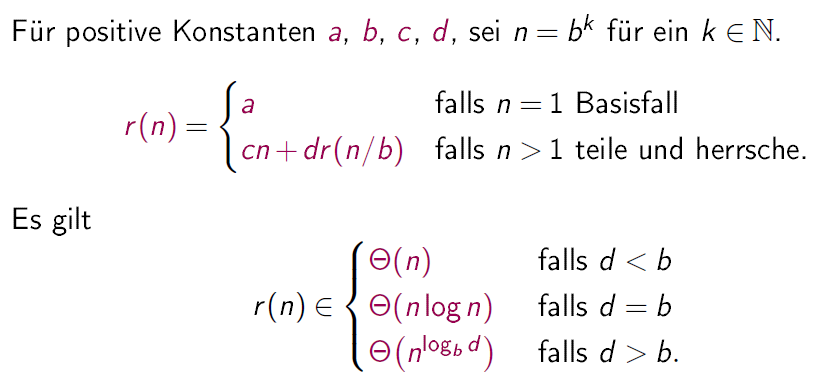
\includegraphics[scale=0.5]{laufzeit/masterTheorem}
\end{frame}

\begin{frame}[t]{MT: Beispiele}
	Wir betrachten verschiedene Sortierverfahren:\\
	\bigskip
	
	\textbf{Mergesort}\\
	msort(L: Liste mit $|L| = n$):\\
	\quad	teile L in der Mitte auf in $L_1$ und $L_2$\\
	\quad	sortiere $L_1$ und $L_2$ mit msort \\
	\quad 	füge $L_1$ und $L_2$ in $\Th{n}$ zusammen\\
	\medskip
	
	$$\text{Laufzeit:} \quad T(n) = \pause \begin{cases}
	1 & n = 1\\
	2 \cdot T(\fract n/2 ) + c \cdot n & n > 1
	\end{cases}$$
	
	\pause
	Nach MT (Fall 2) also: $T(n) \in \Th{n \log n}$.
\end{frame}

\begin{frame}[t]{MT: Beispiele}
	Wir betrachten verschiedene Sortierverfahren:\\
	\bigskip
	
	\textbf{DoubleMergesort}\\
	dmsort(L: Liste mit $|L| = n$):\\
	\quad teile L in der Mitte auf in $L_1$ und $L_2$\\
	\quad sortiere $L_1$ und $L_2$ \textbf{jeweils zwei Mal} mit dmsort\\
	\qquad \textit{Ja, das ist natürlich konstruierter Blödsinn!}\\
	\quad füge $L_1$ und $L_2$ in $\Th{n}$ zusammen\\
	\medskip
	
	$$\text{Laufzeit:} \quad T(n) = \pause \begin{cases}
	1 & n = 1\\
	4 \cdot T(\fract n/2 ) + c \cdot n  & n > 1
	\end{cases}$$
	
	\pause
	Nach MT (Fall 3) also: $T(n) \in \Th{n^{\log_2 4}} = \Th{n^2}$.
\end{frame}

\begin{frame}[t]{MT: Beispiele}
	Wir betrachten verschiedene Sortierverfahren:\\
	\bigskip
	
	\textbf{Magicsort}\\
	magicsort(L: Liste mit $|L| = n$):\\
	\quad teile L in der Mitte auf in $L_1$ und $L_2$\\
	\quad sortiere $L_1$ mit magicsort\\
	\quad sortiere $L_2$ von einem Flaschengeist (in \textbf{Nullkommanichts}!)\\
	\quad füge $L_1$ und $L_2$ in $\Th{n}$ zusammen\\
	\medskip
	
	$$\text{Laufzeit:} \quad T(n) = \pause \begin{cases}
	1 & n = 1\\
	1 \cdot T(\fract n/2 ) + c \cdot n & n > 1
	\end{cases}$$
	
	\pause
	Nach MT (Fall 1) also: $T(n) \in \Th{n}$.
	\medskip
	
	\textbf{ACHTUNG:} Magicsort kann es nicht geben! In Algorithmen I:\\ 
	Untere Schranke für vergleichsbasiertes Sortieren ist $\Om{n \log n}$
\end{frame}


\begin{frame}{Grenzen des MT}
	Nein, das Master-Theorem kann \textbf{nicht} alles (auch wenn es so heißt...). \\
	\smallskip
	\impl Nur verwendbar, wenn die Formeln \textbf{exakt} matchen! (Passiert häufig...) \\
	\smallskip
	In GBI-VL: erweitertes MT (aber auch nicht vollständig!) \\
	\medskip
	Ungleiche Aufteilungen? Vergesst es. \\
	\thasse{Bsp.: \quad Bei der Berechnung von $n! = n \· (n-1)!$ kann die Laufzeit \textbf{nicht} mit dem MT abgeschätzt werden.	}
	
	\mycomment{
		Das Master-Theorem ist mächtig, aber leider längst nicht so mächtig, wie der Name es vielleicht vermuten lässt.\\
		\pause
		Dieses (einfache) MT funktioniert nur bei sehr speziellen Rekurrenzformen (auch wenn diese häufig vorkommen).\\
		\pause
		Ein erweitertes MT wurde in der VL vorgestellt, ist aber auch nicht vollständig!\\
		\pause
		\medskip
		Bei ungleichen Aufteilungen hilft einem das MT überhaupt nicht weiter:\\
		Berechnet man $(n + 1)! = n! \cdot (n + 1)$, so kann die Laufzeit der Berechnung nicht mit dem MT abgeschätzt werden.	
	}
	
	
\end{frame}